\documentclass[10 pt,usenames,dvipsnames, oneside]{article}
\usepackage{../../../modelo-fracoes}
\graphicspath{{../../../Figuras/licao01/}}


\begin{document}

\begin{center}
  \begin{minipage}[l]{3cm}
\includegraphics[width=2cm]{logo}    
\end{minipage}\hfill
\begin{minipage}[r]{.8\textwidth}
 {\Large \scshape Atividade: Oito retângulos: quartos ou só 4 partes?}  
\end{minipage}
\end{center}
\vspace{.2cm}

\ifdefined\prof
\begin{goals}
\begin{enumerate}

    \item       Reconhecer que, em uma equipartição, as partes podem não ter a mesma forma.
    \item       Identificar a equivalência entre as partes de uma equipartição a partir de sobreposição ou da comparação pelo reconhecimento da associação a uma mesma fração unitária (no caso,um quarto).
    \item       Reconhecer a quarta parte como a metade da metade.

\end{enumerate}
\tcblower
\tikzset{x=1cm, y=1cm}
  \begin{itemize} %s
    \item No final deste volume estão disponíveis materiais para reprodução. Cada estudante deve receber os oito retângulos coloridos
    \item Recomenda-se que esta atividade seja desenvolvida em grupos de 3 a 5 alunos.
    \item Caso não seja possível imprimir os retângulos em cores, use a versão em preto e branco, também disponível no final do livro, e peça para os estudantes colorirem. O objetivo das cores é facilitar a identificação dos retângulos na discussão em sala.
    \item É importante observar que todos os retângulos estão divididos em quartos. Conduza a discussão de modo a levar os alunos a reconhecer que, em uma equipartição, as partes não precisam ter a mesma forma.
    \item Nesta atividade, espera-se que os alunos consigam lidar com a figura de um retângulo como representativa de uma unidade genérica.  No entanto, se necessário, o professor pode associar cada retângulo a um objeto concreto (por exemplo, uma barra de chocolate ou a um pedaço de bolo).
    \item É esperado que não seja imediato o reconhecimento de que as partes dos retângulos da segunda linha representam quartos. Nesse caso,  uma alternativa possível é solicitar que eles recortem as partes de cada um dos retângulos da primeira linha para realizar a comparação por sobreposição com as partes dos retângulos da segunda linha.
   \item Recomenda-se ressaltar para os estudantes ao término da atividade que um quarto é a metade da metade.
    \item Em alguns casos, a comparação se dará pela identificação da fração unitária correspondente a cada parte. Nesses casos, o aluno deve reconhecer que a quarta parte é equivalente à metade da metade. Por exemplo, como no caso seguir.
 \begin{center}
 % \centering
 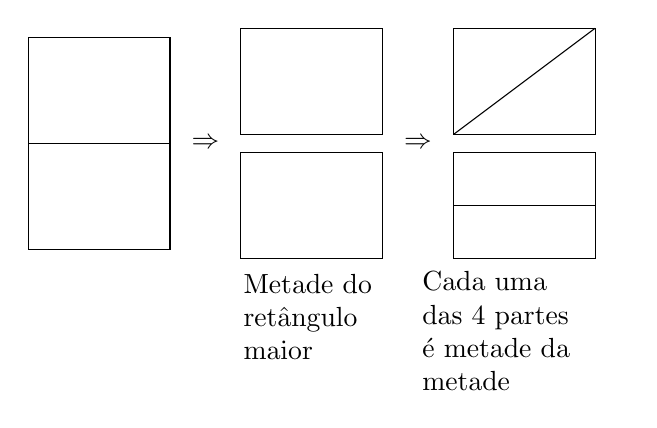
\begin{tikzpicture}[scale=0.45]
  \draw (0,0) rectangle (4,3);
  \draw (0,3) rectangle (4,6);
 % \draw (0,1.5) -- (4,1.5);
  \draw (5,3) node{$\Rightarrow$};
  \draw (6,-0.25) rectangle (10,2.75);
  \draw (6,3.25) rectangle (10,6.25);
  \node[text width=2cm]  at (8.3,-1.9) {Metade do retângulo maior};
  \draw (11,3) node{$\Rightarrow$};
  \draw (12,-0.25) rectangle (16,2.75);
  \draw (12,3.25) rectangle (16,6.25);
  \draw (12,3.25) -- (16,6.25);
  \draw (12,1.25) -- (16,1.25);
  \node[text width=2.5cm]  at (13.9,-2.3) {Cada uma das 4 partes é metade da metade};
  \end{tikzpicture}
\end{center}


\item Segundo a avaliação do professor, a atividade pode ser realizada em duas etapas. Em um primeiro momento, os alunos recebem as primeiras quatro das oito imagens e realizam a atividade com essas imagens - cuja comparação se dá apenas pela sobreposição. Em seguida, recebem as outras quatro, para concluir a atividade. 

\item Da experiência dos autores com a implementação desta atividade em sala de aula, constatou-se uma empolgação dos estudantes quando, ao percebem que formas diferentes podem representar a mesma fração da unidade, foram convidados a gerarem outras equipartições dessa unidade. Seguem outras possíveis equipartições:


  \begin{center}
  
    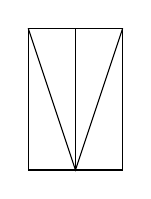
\begin{tikzpicture}[scale=.3]
      \draw[black] (0,0) rectangle (4,6);
      \draw (2,0) -- (2,6);
      \draw (0,6) -- (2,0) -- (4,6);
    \end{tikzpicture}\quad\quad\quad
        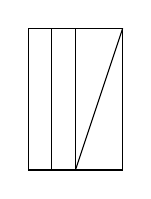
\begin{tikzpicture}[scale=.3]
      \draw[black] (0,0) rectangle (4,6);
      \draw (2,0) -- (2,6);
      \draw (1,0) -- (1,6);
      \draw (2,0) --  (4,6);
    \end{tikzpicture}\quad\quad\quad
        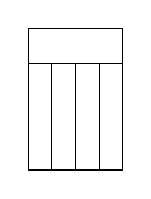
\begin{tikzpicture}[scale=.3]
      \draw[black] (0,0) rectangle (4,6);
      \draw (1,0) -- (1,4.5);
      \draw (2,0) -- (2,4.5);
      \draw (3,0) -- (3,4.5);
      \draw (0,4.5) --  (4,4.5);
    \end{tikzpicture}
  \end{center}
\end{itemize} %s

\end{goals}

\bigskip
\begin{center}
{\huge \scshape Atividade}
\end{center}
\fi

\begin{enumerate} [label=\alph*)] %s
  \item     Quais dos oito retângulos a seguir foram partidos em \textit{quartos}? \newline
 %\vspace{0.2cm}

\begin{center}
 \begin{tikzpicture}[scale=5, x=1mm, y=1mm]
   % primeiro de cima
   % [fill=common, fill opacity=.3]
  \fill[cbpink] (0,0) rectangle (4,6);
  \draw (0,0) rectangle (1,6);
  \draw (1,0) rectangle (2,6);
  \draw (2,0) rectangle (3,6);
  \draw (3,0) rectangle (4,6);
  
  % segundo de cima
  \draw[fill=cbgreen] (5,0) rectangle (9,3);
  \draw[fill=cbgreen] (5,3) rectangle (9,6);
  \draw (5,0) -- (9,3);
  \draw (5,3) -- (9,6);

  \begin{scope}[xshift=28.5, x=1mm, y=1mm]
  % terceiro de cima    
\fill[cbbrown] (0,0) rectangle (4,6);
  \draw(0,0) rectangle (4,1.5);
  \draw (0,1.5) rectangle (4,3);
  \draw (0,3) rectangle (4,4.5);
  \draw (0,4.5) rectangle (4,6);

  % quarto de cima
  \fill[cbolive] (5,0) rectangle (9,6);
  \draw (5,0) rectangle (9,3);
  \draw (5,3) rectangle (9,6);
  \draw (7,0) -- (7,6);

  \end{scope}
  
\end{tikzpicture}

\vspace{0.2cm}

\begin{tikzpicture}[scale=5, x=1mm, y=1mm]

  \begin{scope}[xshift=-28.5]
    % primeiro debaixo
  \fill[cbpurple] (10,0) rectangle (14,6);  
  \draw (10,0) rectangle (14,3);
  \draw (10,3) rectangle (14,6);
  \draw (12,0) -- (12,3);
  \draw (10,4.5) -- (14,4.5);
  
  % 2 debaixo
  %\draw (15,0) rectangle (19,6);
  \filldraw[fill=cbyellow] (15,0) rectangle (19,3);
  \filldraw[fill=cbyellow] (15,3) rectangle (19,6);
  \draw (15,1.5) -- (19,1.5);
 \draw (15,3) -- (19,6);
  \end{scope}
  % 3 debaixo
  \fill[cbgray, opacity=.8] (10,0) rectangle (14,6);
  \draw[fill=cbgray, fill opacity=.3] (10,0) rectangle (14,3);
  \draw[fill=cbgray, fill opacity=.3] (10,3) rectangle (14,6);
  \draw (12,0) -- (12,3);
  \draw (10,6) -- (14,3);

  % 4 debaixo  
  \begin{scope}[xshift=42.5, x=1mm, y=1mm]
  \fill[cborange] (0,0) rectangle (4,6);
  \draw[fill=cborange, fill opacity=.3] (0,0) rectangle (4,6);
  \draw (1,0) -- (1,6);
  \draw (2,0) -- (2,6);
  \draw (2,3) -- (4,3);
  \end{scope}
\end{tikzpicture}
\end{center}

  \item     Desenhe um retângulo e faça uma partição desse retângulo em quatro partes que não sejam todas quartos.
\end{enumerate}

\ifdefined\prof

\begin{solucao}

\begin{enumerate}[label=\alph*),wide,labelindent=0pt] %s
    \item       Todos os retângulos estão divididos em quartos.
    \item       Dois desenhos possíveis são:
\begin{center}
    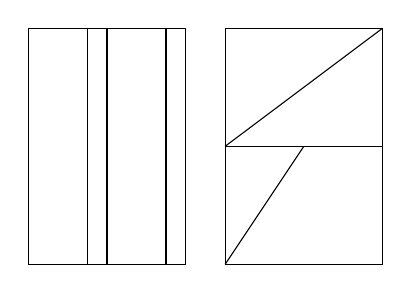
\begin{tikzpicture}[scale=5, x=1mm, y=1mm, every path/.style={black}]
  \draw (0,0) rectangle (1.5,6);
  \draw (1.5,0) rectangle (2,6);
  \draw (2,0) rectangle (3.5,6);
  \draw (3.5,0) rectangle (4,6);
  \draw (5,0) rectangle (9,3);
  \draw (5,3) rectangle (9,6);
  \draw (5,0) -- (7,3);
  \draw (5,3) -- (9,6);
\end{tikzpicture}
\end{center}
\end{enumerate} %s

\end{solucao}
\fi

\end{document}